\documentclass[gr-notes.tex]{subfiles}

\begin{document}

\setcounter{chapter}{1}

\chapter{Vector analysis in special relativity}

\section{Definition of a vector}

\section{Vector algebra}

\section{The four-velocity}

An object's four velocity, denoted $\vec{U}$, is the vector tangent to its world line, with unit length. This means it extends one unit in time, and zero in space, so it is timelike.

For an \emph{accelerated} particle (which we have not considered up to now), we may not be able to define an inertial frame, but we \emph{can} define a \textbf{momentarily comoving reference frame} (MCRF) which, as the name suggests, moves with the same velocity as the observer for an infinitesimal period of time. We can therefore construct a continuous sequence of MCRFs for any object. If an object has MCRF $\obs$, then its four-velocity is \emph{defined} to be the basis vector $\vec{e}_0$.


\section{The four-momentum}

Analogous to the three-momentum, we define the four-momentum to be
%
\begin{displaymath}
  \vec{p} = m \vec{U}.
%
  \tag{Schutz 2.19}
  \label{schutz:2.19}
\end{displaymath}
%
It has components
%
\begin{displaymath}
  \vec{p} \underset{\obs}{\to} (E, p^1, p^2, p^3).
%
  \tag{Schutz 2.20}
  \label{schutz:2.20}
\end{displaymath}
%
Calling $p^0$ ``$E$'' is no accident, it is in fact the energy. There is an interesting consequence to this: since vectors are invariant with respect to reference frame, but vector components are not, this means that the four-momentum does not change in different reference frames, but the energy \emph{does}. One example would be the doppler effect, which causes the color (or energy) of a photon to shift depending on the radial velocity of the source and observer.



\section{Scalar product}

\begin{displaymath}
  \vec{A} \cdot \vec{B} =
  -(A^0 B^0) + (A^1 B^1) + (A^2 B^2) + (A^3 B^3)
\end{displaymath}

\section{Applications}

\section{Photons}

$\vec{x} \cdot \vec{x} = 0$, so we cannot define $\vec{U}$ for photons. We can, however, define $\vec{p}$. Since $\vec{p} \cdot \vec{p} = -m^2$, and photons are massless, we have $\vec{p} \cdot \vec{p} = 0$.

\section{Further reading}

\section{Exercises}

\textbf{2}
Identify the free and dummy indices in the following equations, and write equivalent expressions with different indices. Also, write how many equations are represented by each expression.

\emph{Note, I will express the set of free indices by $\mathcal{F}$ and the set of dummy indices as $\mathcal{D}$, and I will use the original index names.}

\begin{enumerate}[(a)]
\item $\tensor{A}{^\alpha} \tensor{B}{_\beta} = 5 \implies
       \tensor{A}{^\beta} \tensor{B}{_\alpha} = 5$
      (16 equations,
       $\mathcal{F} = \{ \alpha, \beta \}$,
       $\mathcal{D} = \O$)

\item $\tensor{A}{^{\bar\mu}} =
       \tensor{\Lambda}{^{\bar\mu}_\nu} \tensor{A}{^\nu} \implies
       \tensor{A}{^{\bar\nu}} =
       \tensor{\Lambda}{^{\bar\nu}_\mu} \tensor{A}{^\mu}$
      (4 equations,
       $\mathcal{F} = \{ \bar\mu \}$,
       $\mathcal{D} = \{ \nu \}$).

\item $\tensor{T}{^{\alpha\mu\lambda}}
       \tensor{A}{_\mu}
       \tensor{C}{_\lambda^\gamma} =
       \tensor{D}{^{\gamma\alpha}} \implies
       \tensor{T}{^{\eta\phi\theta}}
       \tensor{A}{_\phi}
       \tensor{C}{_\theta^\zeta} =
       \tensor{D}{^{\zeta\eta}}$
      (16 equations,
       $\mathcal{F} = \{ \alpha, \gamma \}$,
       $\mathcal{D} = \{ \mu, \lambda \}$)

\item $\tensor{R}{_{\mu\nu}} - \frac{1}{2} \tensor{g}{_{\mu\nu}} =
       \tensor{G}{_{\mu\nu}} \implies
       \tensor{R}{_{\chi\epsilon}} - \frac{1}{2} \tensor{g}{_{\chi\epsilon}} =
       \tensor{G}{_{\chi\epsilon}}$
      (16 equations,
       $\mathcal{F} = \{ \mu, \nu \}$,
       $\mathcal{D} = \O$)
\end{enumerate}


\textbf{4}
Given vectors $\vec{A} \to_\obs (5, -1, 0, 1)$ and $\vec{B} \to_\obs (-2, 1, 1, -6)$, find the components in $\obs$ of

\begin{enumerate}[(a)]
\item $-6\vec{A} \to_\obs (-30, 6, 0, -6)$

\item $3\vec{A} + \vec{B} \to_\obs (13, -2, 1, -3)$

\item $-6\vec{A} + 3\vec{B} \to_\obs (-36, 9, 3, -24)$
\end{enumerate}


\textbf{6}
Draw a spacetime diagram from $\obs$'s reference frame. There are two other frames, $\bar\obs$ and $\bar{\bar\obs}$, which are each moving with velocity $0.6$ in the $+x$ direction from each respective frame. Plot each frame's basis vectors, as observed by $\obs$.

See Figure \ref{fig:exercise-6}.

\begin{figure}[h]
  \centering
  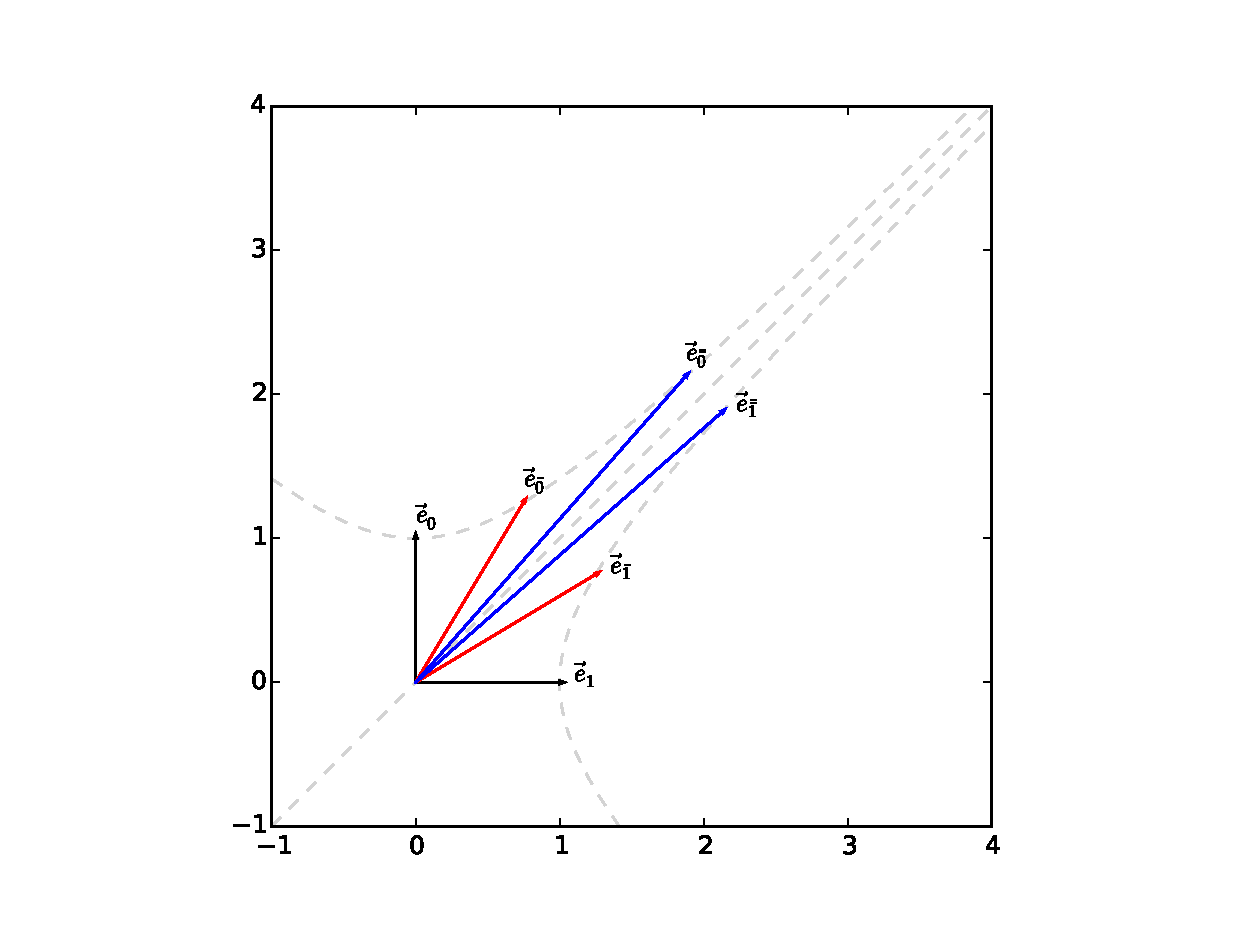
\includegraphics[width=0.9\textwidth]{img/problem6}
  \caption{Exercise 6}
  \label{fig:exercise-6}
\end{figure}


\textbf{9}
Prove, by writing out all the terms that
%
\begin{displaymath}
  \sum_{\bar\alpha = 0}^3 \qty(
    \sum_{\beta = 0}^3
      \tensor{\Lambda}{^{\bar\alpha}_\beta}
      \tensor{A}{^\beta}
      \vec{e}_{\bar\alpha}
  ) =
  \sum_{\beta = 0}^3 \qty(
    \sum_{\bar\alpha = 0}^3
      \tensor{\Lambda}{^{\bar\alpha}_\beta}
      \tensor{A}{^\beta}
      \vec{e}_{\bar\alpha}
  )
\end{displaymath}
%
\begin{align*}
  \sum_{\bar\alpha = 0}^3 \qty(
    \sum_{\beta = 0}^3
      \tensor{\Lambda}{^{\bar\alpha}_\beta}
      \tensor{A}{^\beta}
      \vec{e}_{\bar\alpha}
  ) &=
  \sum_{\bar\alpha = 0}^3 \qty(
    \tensor{\Lambda}{^{\bar\alpha}_0} \tensor{A}{^0} \vec{e}_{\bar\alpha} +
    \tensor{\Lambda}{^{\bar\alpha}_1} \tensor{A}{^1} \vec{e}_{\bar\alpha} +
    \tensor{\Lambda}{^{\bar\alpha}_2} \tensor{A}{^2} \vec{e}_{\bar\alpha} +
    \tensor{\Lambda}{^{\bar\alpha}_3} \tensor{A}{^3} \vec{e}_{\bar\alpha}
  )
  \\ &=
  \tensor{\Lambda}{^{\bar0}_0} \tensor{A}{^0} \vec{e}_{\bar0} +
  \tensor{\Lambda}{^{\bar0}_1} \tensor{A}{^1} \vec{e}_{\bar0} +
  \tensor{\Lambda}{^{\bar0}_2} \tensor{A}{^2} \vec{e}_{\bar0} +
  \tensor{\Lambda}{^{\bar0}_3} \tensor{A}{^3} \vec{e}_{\bar0}
  \\ &+
  \tensor{\Lambda}{^{\bar1}_0} \tensor{A}{^0} \vec{e}_{\bar1} +
  \tensor{\Lambda}{^{\bar1}_1} \tensor{A}{^1} \vec{e}_{\bar1} +
  \tensor{\Lambda}{^{\bar1}_2} \tensor{A}{^2} \vec{e}_{\bar1} +
  \tensor{\Lambda}{^{\bar1}_3} \tensor{A}{^3} \vec{e}_{\bar1}
  \\ &+
  \tensor{\Lambda}{^{\bar2}_0} \tensor{A}{^0} \vec{e}_{\bar2} +
  \tensor{\Lambda}{^{\bar2}_1} \tensor{A}{^1} \vec{e}_{\bar2} +
  \tensor{\Lambda}{^{\bar2}_2} \tensor{A}{^2} \vec{e}_{\bar2} +
  \tensor{\Lambda}{^{\bar2}_3} \tensor{A}{^3} \vec{e}_{\bar2}
  \\ &+
  \tensor{\Lambda}{^{\bar3}_0} \tensor{A}{^0} \vec{e}_{\bar3} +
  \tensor{\Lambda}{^{\bar3}_1} \tensor{A}{^1} \vec{e}_{\bar3} +
  \tensor{\Lambda}{^{\bar3}_2} \tensor{A}{^2} \vec{e}_{\bar3} +
  \tensor{\Lambda}{^{\bar3}_3} \tensor{A}{^3} \vec{e}_{\bar3}
  \\ &=
  \tensor{\Lambda}{^{\bar0}_0} \tensor{A}{^0} \vec{e}_{\bar0} +
  \tensor{\Lambda}{^{\bar1}_0} \tensor{A}{^0} \vec{e}_{\bar1} +
  \tensor{\Lambda}{^{\bar2}_0} \tensor{A}{^0} \vec{e}_{\bar2} +
  \tensor{\Lambda}{^{\bar3}_0} \tensor{A}{^0} \vec{e}_{\bar3}
  \\ &+
  \tensor{\Lambda}{^{\bar0}_1} \tensor{A}{^1} \vec{e}_{\bar0} +
  \tensor{\Lambda}{^{\bar1}_1} \tensor{A}{^1} \vec{e}_{\bar1} +
  \tensor{\Lambda}{^{\bar2}_1} \tensor{A}{^1} \vec{e}_{\bar2} +
  \tensor{\Lambda}{^{\bar3}_1} \tensor{A}{^1} \vec{e}_{\bar3}
  \\ &+
  \tensor{\Lambda}{^{\bar0}_2} \tensor{A}{^2} \vec{e}_{\bar0} +
  \tensor{\Lambda}{^{\bar1}_2} \tensor{A}{^2} \vec{e}_{\bar1} +
  \tensor{\Lambda}{^{\bar2}_2} \tensor{A}{^2} \vec{e}_{\bar2} +
  \tensor{\Lambda}{^{\bar3}_2} \tensor{A}{^2} \vec{e}_{\bar3}
  \\ &+
  \tensor{\Lambda}{^{\bar0}_3} \tensor{A}{^3} \vec{e}_{\bar0} +
  \tensor{\Lambda}{^{\bar1}_3} \tensor{A}{^3} \vec{e}_{\bar1} +
  \tensor{\Lambda}{^{\bar2}_3} \tensor{A}{^3} \vec{e}_{\bar2} +
  \tensor{\Lambda}{^{\bar3}_3} \tensor{A}{^3} \vec{e}_{\bar3}
  \\ &=
  \sum_{\beta = 0}^3 \qty(
    \tensor{\Lambda}{^{\bar0}_\beta} \tensor{A}{^\beta} \vec{e}_{\bar0} +
    \tensor{\Lambda}{^{\bar1}_\beta} \tensor{A}{^\beta} \vec{e}_{\bar1} +
    \tensor{\Lambda}{^{\bar2}_\beta} \tensor{A}{^\beta} \vec{e}_{\bar2} +
    \tensor{\Lambda}{^{\bar3}_\beta} \tensor{A}{^\beta} \vec{e}_{\bar3}
  )
  \\ &=
  \sum_{\beta = 0}^3 \qty(
    \sum_{\bar\alpha = 0}^3
      \tensor{\Lambda}{^{\bar\alpha}_\beta}
      \tensor{A}{^\beta}
      \vec{e}_{\bar\alpha}
  )
\end{align*}


\textbf{11}
Let $\tensor{\Lambda}{^{\bar\alpha}_\beta}$ be the matrix of the Lorentz transformation from $\obs$ to $\bar\obs$, given in Equation 1.12. Let $\vec{A}$ be an arbitrary vector with components $(A^0, A^1, A^2, A^3)$ in frame $\obs$.
%
\begin{enumerate}[(a)]
\item Write down the matrix of $\tensor{\Lambda}{^\nu_{\bar\mu}}(-v)$.

Intuitively, it should appear the same as $\tensor{\Lambda}{^{\bar\alpha}_\beta}$, but with the negative signs removed. More rigorously, it is given by the matrix inverse of $\tensor{\Lambda}{^{\bar\alpha}_\beta}$, as their product should be the identity matrix. I have used a computer algebra system (Wolfram Alpha) to take the inverse of this matrix symbolically, confirming my suspicion:
%
\begin{displaymath}
  \tensor{\Lambda}{^\nu_{\bar\mu}}(-v) =
  \mqty(
    \gamma  & v\gamma & 0 & 0
    \\
    v\gamma & \gamma  & 0 & 0
    \\
    0       & 0       & 1 & 0
    \\
    0       & 0       & 0 & 1
  ).
\end{displaymath}

\item Find $\tensor{A}{^{\bar\alpha}}$ for all $\bar\alpha$.

\begin{align*}
  \tensor{A}{^{\bar\alpha}} &=
  \tensor{\Lambda}{^{\bar\alpha}_\beta} \tensor{A}{^\beta}
  \\
  \tensor{A}{^{\bar0}} &= \gamma (\tensor{A}{^0} - v \tensor{A}{^1})
  \\
  \tensor{A}{^{\bar1}} &= \gamma (\tensor{A}{^1} - v \tensor{A}{^0})
  \\
  \tensor{A}{^{\bar2}} &= \tensor{A}{^2}
  \\
  \tensor{A}{^{\bar3}} &= \tensor{A}{^3}
\end{align*}

\item Verify Equation 2.18 by performing the sum for all values of $\nu$ and $\alpha$.

To simplify things, I do this via matrix multiplication
%
\begin{align*}
  \tensor{\Lambda}{^{\bar\alpha}_\beta}(v)
  \tensor{\Lambda}{^\nu_{\bar\mu}}(-v) &=
  \mqty(
    \gamma^2 - v^2 \gamma^2 & v \gamma^2 - v \gamma^2 & 0 & 0
    \\
    v \gamma^2 - v \gamma^2 & \gamma^2 - v^2 \gamma^2 & 0 & 0
    \\
    0 & 0 & 1 & 0
    \\
    0 & 0 & 0 & 1
  )
  \\ &=
  \mqty(
    \gamma^2 (1 - v^2) & 0 & 0 & 0
    \\
    0 & \gamma^2 (1 - v^2) & 0 & 0
    \\
    0 & 0 & 1 & 0
    \\
    0 & 0 & 0 & 1
  )
  \\ &=
  \mqty(\imat{4}) =
  \tensor{\delta}{^\nu_\alpha}
\end{align*}

\item Write down the Lorentz transformation matrix from $\bar\obs$ to $\obs$, justifying each term.

It should just be $\tensor{\Lambda}{^\nu_{\bar\mu}}(-v)$. I'm not sure what else to say at this point.

\item Using the result from part (d), find $A^\beta$ from $A^{\bar\alpha}$. How does this relate to Equation 2.18?

\begin{align*}
  \tensor{\Lambda}{^\beta_{\bar\alpha}} A^{\bar\alpha} &=
  \mqty(  \gamma & v \gamma & 0 & 0 \\
        v \gamma &   \gamma & 0 & 0 \\
               0 &        0 & 1 & 0 \\
               0 &        0 & 0 & 1)
  \mqty(\gamma (A^0 - v A^1) \\
        \gamma (A^1 - v A^0) \\
        A^2 \\
        A^3) =
  \mqty(  \gamma^2 (A^0 - v A^1) + v \gamma^2 (A^1 - v A^0) + 0 + 0 \\
        v \gamma^2 (A^0 - v A^1) +   \gamma^2 (A^1 - v A^0) + 0 + 0 \\
        A^2 \\
        A^3)
  \\ &=
  \mqty(A^0 (  \gamma^2 - v^2 \gamma^2) + A^1 (v \gamma^2 - v \gamma^2) \\
        A^0 (v \gamma^2 - v^2 \gamma^2) + A^1 (  \gamma^2 - v \gamma^2) \\
        A^2 \\
        A^3) =
  \mqty(A^0 (\gamma^2 - v^2 \gamma^2) \\
        A^1 (\gamma^2 - v^2 \gamma^2) \\
        A^2 \\
        A^3) =
  \mqty(A^0 \\ A^1 \\ A^2 \\ A^3) =
  A^\beta
\end{align*}

Since $A^{\bar\alpha} = \tensor{\Lambda}{^{\bar\alpha}_\beta}(v)$, this goes to show that $\tensor{\Lambda}{^\nu_{\bar\beta}}(-v) \tensor{\Lambda}{^{\bar\beta}_\alpha}(-v) A^\lambda = A^\lambda \implies \tensor{\Lambda}{^\nu_{\bar\beta}}(-v) \tensor{\Lambda}{^{\bar\beta}_\alpha}(-v) = \tensor{\delta}{^\nu_\alpha}$.

\item Verify in the same manner as (c) that

  \begin{displaymath}
    \tensor{\Lambda}{^\nu_{\bar\beta}}(v)
    \tensor{\Lambda}{^{\bar\alpha}_\nu}(-v) =
    \tensor{\delta}{^{\bar\alpha}_{\bar\beta}}
  \end{displaymath}

  My matrix multiplication approach will just give me the same result as before. Perhaps another approach was intended?


\item Establish that

  \begin{align*}
    \vec{e}_\alpha &=
    \tensor{\Lambda}{^{\bar\beta}_\alpha} \vec{e}_{\bar\beta} =
    \tensor{\Lambda}{^{\bar\beta}_\alpha} \tensor{\Lambda}{^\nu_{\bar\beta}}
    \vec{e}_\nu =
    \tensor{\delta}{^\nu_\alpha} \vec{e}_\nu
    \\
    A^{\bar\beta} &=
    \tensor{\Lambda}{^{\bar\beta}_\alpha} A^\alpha =
    \tensor{\Lambda}{^{\bar\beta}_\alpha} \tensor{\Lambda}{^\alpha_{\bar\mu}}
    A^{\bar\mu} =
    \tensor{\delta}{^{\bar\beta}_{\bar\mu}} A^{\bar\mu}
  \end{align*}


\end{enumerate}



\textbf{14}
The following matrix gives a Lorentz transformation from $\obs$ to $\bar\obs$:
\begin{displaymath}
  \mqty(
    1.25 & 0 & 0 & 0.75
    \\
    0 & 1 & 0 & 0
    \\
    0 & 0 & 1 & 0
    \\
    0.75 & 0 & 0 & 1.25
  )
\end{displaymath}


\begin{enumerate}[(a)]

\item What is the velocity of $\bar\obs$ relative to $\obs$?

This would correspond to a Lorentz boost along the $z$-axis, meaning
%
\begin{displaymath}
  \tensor{\Lambda}{^{\bar\alpha}_\beta}(v) =
  \mqty(
    \gamma & 0 & 0 & -v\gamma
    \\
    0 & 1 & 0 & 0
    \\
    0 & 0 & 1 & 0
    \\
    -v\gamma & 0 & 0 & \gamma
  ),
\end{displaymath}
%
and thus we have $\gamma = 1.25$ and $-v\gamma = 0.75$. Solving for $v$, we get
%
\begin{displaymath}
  -v \gamma =
  \frac{3}{4} \implies
  v =
  -\frac{3}{4 \gamma} =
  -\frac{3 \cdot 4}{4 \cdot 5} =
  -\frac{3}{5}.
\end{displaymath}
%
So $\bar\obs$ is moving with speed $0.6$ relative to the $-z$-axis of $\obs$.

\item What is the inverse matrix to the given one?

Numerically, it comes out to be
\begin{displaymath}
  \mqty(
    1.25 & 0 & 0 & -0.75
    \\
    0 & 1 & 0 & 0
    \\
    0 & 0 & 1 & 0
    \\
    -0.75 & 0 & 0 & 1.25
  ),
\end{displaymath}
which makes sense, when you consider that the inverse matrix should be a Lorentz transformation with the velocity negated.

\item Find the components in $\obs$ of $\vec{A} \to_{\bar\obs} (1, 2, 0, 0)$.
%
\begin{displaymath}
  \vec{A} \underset{\obs}{\to}
  \mqty(
    1.25 & 0 & 0 & -0.75
    \\
    0 & 1 & 0 & 0
    \\
    0 & 0 & 1 & 0
    \\
    -0.75 & 0 & 0 & 1.25
  )
  \mqty( 1 \\ 2 \\ 0 \\ 0 ) =
  \mqty( 1.25 \\ 2 \\ 0 \\ -0.75 )
\end{displaymath}

\end{enumerate}

\textbf{15}

\begin{enumerate}[(a)]
\item Compute the four-velocity components in $\obs$ of a particle whose speed is $v$ in the $+x$-direction relative to $\obs$, using the Lorentz transformation.
%
\begin{align*}
  \vec{U} &= \vec{e}_{\bar0}
  \\
  \tensor{U}{^\alpha} &=
  \tensor{\Lambda}{^\alpha_{\bar\beta}} (\vec{e}_{\bar0})^{\bar\beta} =
  \Lambda^\alpha_{\bar0},
  \\
  U^0 &= \gamma
  \\
  U^1 &= v \gamma
  \\
  U^2 &= U^3 = 0
\end{align*}

\item Generalize to arbitrary velocities $\boldsymbol{v}$, where $\abs{v} < 1$.

\begin{align*}
  \tensor{\Lambda}{^\alpha_{\bar\beta}}(\boldsymbol{v}) &=
  \mqty(\gamma     & \gamma v_x & \gamma v_y & \gamma v_z \\
        \gamma v_x & \gamma     & 0          & 0          \\
        \gamma v_y & 0          & \gamma     & 0          \\
        \gamma v_z & 0          & 0          & \gamma     ).
  \\
  U^0 &= \gamma
  \quad
  U^1 = \gamma v_x
  \quad
  U^2 = \gamma v_y
  \quad
  U^3 = \gamma v_z
\end{align*}


% Consider three Lorentz boosts, one along each of the $x$, $y$, and $z$ axes. We can accomplish this by imagining an observer $\bar\obs$, moving at a velocity $v_x$ relative to $\obs$'s $x$-axis. Then imagine another observer, $\bar{\bar\obs}$, moving at a velocity $v_y$ along $\bar\obs$'s $y$-axis. Finally, imagine an observer $\bar{\bar{\bar\obs}}$, moving at a velocity $v_z$ aong $\bar{\bar\obs}$'s $z$-axis. The total Lorentz transformation can be written by
% %
% \begin{displaymath}
%   \tensor{U}{^{\bar{\bar{\bar\alpha}}}} =
%   \tensor{\Lambda}{^{\bar{\bar{\bar\alpha}}}_{\bar{\bar\beta}}}(v_z)
%   \tensor{\Lambda}{^{\bar{\bar{\beta}}}_{\bar\gamma}}(v_y)
%   \tensor{\Lambda}{^{\bar\gamma}_\delta}(v_x)
%   \tensor{U}{^\delta} =
%   \tensor{\Lambda}{^{\bar{\bar{\bar\alpha}}}_\delta}(\boldsymbol{v})
%   \tensor{U}{^\delta}
% \end{displaymath}

\item Use this result to express $\boldsymbol{v}$ as a function of the components $\{ U^\alpha \}$.

\begin{align*}
  \boldsymbol{v} &=
  v_x \vec{e}_1 + v_y \vec{e}_2 + v_z \vec{e}_3
  \\
  v_i &= \frac{U^i}{\gamma}
  \\
  \boldsymbol{v} &= \frac{1}{\gamma} U^i \vec{e}_i
\end{align*}

\item Find the three-velocity $\boldsymbol{v}$ of a particle with four-velocity components $(2, 1, 1, 1)$.

$U^0 = \gamma = 2$, and $U^i = 1$, so
%
\begin{displaymath}
  \boldsymbol{v} = \frac{1}{2} \vec{e}_i
\end{displaymath}


\end{enumerate}


\textbf{17}

\textbf{Not sure how to approach this problem.}

\begin{enumerate}[(a)]
\item Prove that any timelike vector $\vec{U}$ for which $U^0 > 0$ and $\vec{U} \cdot \vec{U} = -1$ is the four-velocity of \emph{some} world line.


\item Use this to prove that for any timelike vector $\vec{V}$ there is a Lorentz frame in which the $\vec{V}$ has zero spatial components.
\end{enumerate}


\textbf{19}
A body is uniformly accelerated if the four-vector $\vec{a}$ has constant spatial direction and magnitude, $\vec{a} \cdot \vec{a} = \alpha^2 \geq 0$.

(a) Show that this implies the components of $\vec{a}$ in the body's MCRF are all constant, and that these are equivalent to the Galilean ``acceleration''.

We normalize the vector $\vec{a}$ by dividing each of its terms by the magnitude of the vector, so
%
\begin{displaymath}
  \frac{a^\lambda}{\alpha}.
\end{displaymath}
%
Since $\alpha$ is constant, and also the \emph{direction} is constant, this means that the above expression is \emph{also} constant, as the normalized components tell you about the direction. If we multiply a constant by a constant, we should still get a constant, so we multiply the above expression by $\alpha$, getting $a^\lambda$ to be constant.

In the MCRF of an object, $\dd\tau = \dd{t}$, and so we can write
%
\begin{displaymath}
  \vec{a} = \dv{\vec{U}}{t} = \qty(0, \dv{U^1}{t}, \dv{U^2}{t}, \dv{U^3}{t}),
\end{displaymath}
%
which is analogous to the Galilean acceleration.

(b) A body is uniformly accelerated with $\alpha = \SI{10}{\meter\per\second^2}$. It starts from rest, and falls for a time $t$. Find its speed as a function of $t$, and find the time to reach $v = 0.999$.

\begin{align*}
  \vec{U} &\underset{\rm MCRF}{\to}
  (1, 0, 0, 0)
  \\ &\underset{\obs}{\to}
  (\gamma, \gamma v, 0, 0)
  \\
  \dv{\vec{U}}{\tau} &\underset{\rm MCRF}{\to}
  (0, \alpha, 0, 0)
  \\ &\underset{\obs}{\to}
  (\gamma, \gamma \alpha, 0, 0)
  \\
  U^x &=
  \int_0^t \dv{U^x}{\tau} \dd\tau =
  \int_0^t \gamma \alpha \frac{\dd{t}}{\gamma} =
  \int_0^t \alpha \dd{t} =
  \alpha t
  \\ &=
  \gamma v =
  \frac{v}{\sqrt{1 - v^2}}
  \\
  v^2 &=
  (\alpha t)^2 (1 - v^2) =
  (\alpha t)^2 - (\alpha t v)^2
  \\
  v^2 (1 + (\alpha t)^2) &=
  (\alpha t)^2
  \\
  v^2 &=
  \frac{(\alpha t)^2}{1 + (\alpha t)^2} \implies
  v = \sqrt{\frac{(\alpha t)^2}{1 + (\alpha t)^2}}
\end{align*}
%
To find the time to reach $v = 0.999$, we go back to the expression $\gamma v = \alpha t$, solve for $t$, and substitute for $v$ and $\alpha$. Note that in natural units, $\alpha = \SI{10}{\meter\per\second^2} c^{-2} \approx \SI{1.11e-16}{\per\meter}$
%
\begin{align*}
  t &=
  \frac{v}{\alpha \sqrt{1 - v^2}} =
  \frac{0.999}{\SI{1.11e-16}{\per\meter} \sqrt{1 - 0.999^2}} \approx
  \SI{2.01e17}{\meter}.
\end{align*}



\textbf{24}
Show that a positron and electron cannot annihilate to form a single photon, but they can annihilate to form two photons.

We consider the center of momentum frame, where $\sum \vec{p}_{(i)} \to_{\mathrm{CM}} (E_{\mathrm{total}}, 0, 0, 0)$. Without loss of generality, we assume that the velocities of the two particles are equal and opposite, such that
%
\begin{align*}
  \vec{p}_{e^+} &\to_{\mathrm{CM}} m_e (\gamma,  \gamma v, 0, 0), &
  \vec{p}_{e^-} &\to_{\mathrm{CM}} m_e (\gamma, -\gamma v, 0, 0).
\end{align*}
%
The photon they create will have to have a momentum of $\vec{p}_{\gamma,\mathrm{single}} \to_{\mathrm{CM}} (h \nu, h \nu, 0, 0)$. By conservation of four-momentum, we have
%
\begin{align*}
  \vec{p}_{e^+} + \vec{p}_{e^-} &= \vec{p}_{\gamma,\mathrm{single}}
  \\
  (\vec{p}_{e^+} + \vec{p}_{e^-}) \cdot (\vec{p}_{e^+} + \vec{p}_{e^-}) &=
  \vec{p}_{\gamma,\mathrm{single}} \cdot \vec{p}_{\gamma,\mathrm{single}}
  \\
  (\vec{p}_{e^+} \cdot \vec{p}_{e^+}) +
  (\vec{p}_{e^-} \cdot \vec{p}_{e^-}) +
  (\vec{p}_{e^+} \cdot \vec{p}_{e^-}) &=
  0
  \\
  -m_e^2 - m_e^2 - m_e^2 &= 0
  \implies m_e = 0!
\end{align*}
%
Since we know that $m_e$ is in fact non-zero, this cannot possibly happen.

Now consider the scenario wherein two photons are created, moving in opposite directions. Then they would have momenta: $\vec{p}_{\gamma,1} \to_{\mathrm{CM}} (h \nu, h \nu, 0, 0)$ and $\vec{p}_{\gamma,2} \to_{\mathrm{CM}} (h \nu, -h \nu, 0, 0)$. Invoking conservation of four-momentum as before, we get
%
\begin{align*}
  \vec{p}_{e^+} + \vec{p}_{e^-} &= \vec{p}_{\gamma,1} + \vec{p}_{\gamma,2}
  \\
  (\vec{p}_{e^+} + \vec{p}_{e^-}) \cdot
  (\vec{p}_{e^+} + \vec{p}_{e^-}) &=
  (\vec{p}_{\gamma,1} + \vec{p}_{\gamma,2}) \cdot
  (\vec{p}_{\gamma,1} + \vec{p}_{\gamma,2})
  \\
  -3 m_e^2 &=
  (\vec{p}_{\gamma,1} \cdot \vec{p}_{\gamma,1}) +
  (\vec{p}_{\gamma,1} \cdot \vec{p}_{\gamma,2}) +
  (\vec{p}_{\gamma,2} \cdot \vec{p}_{\gamma,2})
  \\ &=
  0 + (-h^2 \nu^2 - h^2 \nu^2) + 0 =
  -2 h^2 \nu^2,
\end{align*}
%
so we end up with $3 m_e^2 = 2 h^2 \nu^2$, meaning two photons are produced with $E^2 = \frac{3}{2} m_e^2$, which is entirely reasonable.




\textbf{25}

(a) Consider a frame $\bar\obs$ moving with a speed $v$ along the $x$-axis of $\obs$. Now consider a photon moving at an angle $\theta$ from $\obs$'s $x$-axis. Find the ratio of its frequency in $\bar\obs$ and in $\obs$.

We must first construct the particle's four-momentum. In the case where the photon was moving along the $x$-axis (see Section 2.7), it had been found that the four-momentum was
%
\begin{displaymath}
  \vec{p} \underset{\obs}{\to} (E, E, 0, 0),
\end{displaymath}
%
as this satisfied
%
\begin{displaymath}
  \vec{p} \cdot \vec{p} =
  -E^2 + E^2 =
  0.
%
  \tag{Schutz 2.37}
  \label{schutz:2.37}
\end{displaymath}
%
Now that the photon is moving at an angle $\theta$ from the $x$-axis, we need to redistribute the 3-momentum accordingly. No specification was given as photon's angle in the $y$- or $z$-axis, so without loss of generality, I assume it is constrained to the $x$-$y$ plane. This means we can write the four-momentum as
%
\begin{displaymath}
  \vec{p} \underset{\obs}{\to} (E, E \cos\theta, E \sin\theta, 0),
\end{displaymath}
%
which you can easily confirm satisfies $\vec{p} \cdot \vec{p} = 0$.

Now we may apply the Lorentz transformation $\tensor{\Lambda}{^{\bar0}_\alpha}(v)$ to find the photon's energy as observed by $\bar\obs$, and from that the frequency.
%
\begin{align*}
  p^{\bar0} =
  \bar{E} &=
  \tensor{\Lambda}{^{\bar0}_\alpha} p^\alpha =
  \gamma p^0 - v \gamma p^1 + 0 + 0 =
  \gamma E - v \gamma E \cos\theta
  \\ \implies
  h \bar\nu &=
  \gamma h \nu - v \gamma h \nu \cos\theta
  \\ \implies
  \frac{\bar\nu}{\nu} &=
  \gamma - v \gamma \cos\theta =
  \frac{1 - v \cos\theta}{\sqrt{1 - v^2}}
\end{align*}


(b) Even when the photon moves perpendicular to the $x$-axis ($\theta = \pi/2$) there is a frequency shift. This is the \emph{transverse Doppler shift}, which is a result of time dilation. At which angle $\theta$ must the photon move such that there is no Doppler shift between $\obs$ and $\bar\obs$?

To do this, we simply set $\bar\nu / \nu = 1$, and solve for $\theta$.
%
\begin{align*}
  1 &=
  \frac{1 - v \cos\theta}{\sqrt{1 - v^2}} \implies
  \cos\theta = 1 - \sqrt{1 - v^2}
  \\ \implies
  \theta &=
  \pm \arccos(1 - \sqrt{1 - v^2})
\end{align*}

(c) Now use Equations 2.35 and 2.38 to find $\bar\nu / \nu$.

Recall that $\vec{U} \to_\obs (\gamma, v \gamma, 0, 0)$. Using Equation 2.35 we have
%
\begin{align*}
  \bar{E} =
  h \bar\nu &=
  -(E, E \cos\theta, E \sin\theta, 0) \cdot (\gamma, v \gamma, 0, 0)
  \\ &=
  -(-(E \gamma) + E \gamma v \cos\theta) =
  E \gamma (1 - v \cos \theta) =
  h \nu \gamma (1 - v \cos \theta)
  \\
  \frac{\bar\nu}{\nu} &=
  \frac{1 - v \cos\theta}{\sqrt{1 - v^2}}
\end{align*}





\textbf{26}
Calculate the energy required to accelerate a particle of rest mass $m > 0$ from speed $v$ to speed $v + \var{v}$ ($\var{v} \ll v$), to first order in $\var{v}$. Show that it would take infinite energy to accelerate to $c$.

From the four-momentum we have $E_v = m \gamma$, and from that
%
\begin{displaymath}
  E_{v + \var{v}} = \frac{m}{\sqrt{1 - (v + \var{v})^2}}.
\end{displaymath}
%
If we do a Taylor expansion on $(1 - (v + \var{v})^2)^{-1/2}$ we get
%
\begin{displaymath}
  \frac{1}{\sqrt{1 - v^2}} +
  \frac{v \var{v}}{(1 - v^2)^{3/2}} +
  \order{v^2},
\end{displaymath}
%
so
\begin{align*}
  E_{v + \var{v}} &\approx
  \frac{m}{\sqrt{1 - v^2}} +
  \frac{m v \var{v}}{(1 - v^2)^{3/2}}
  \\
  \Delta E &=
  E_{v + \var{v}} - E_v \approx
  \frac{m v \var{v}}{(1 - v^2)^{3/2}} =
  m \gamma^3 v \var{v}.
\end{align*}
%
As $v \to c$, $\gamma \to \infty$ and therefore $\Delta E \to \infty$.



\textbf{30}
A rocket ship has four-velocity $\vec{U} \to_\obs (2, 1, 1, 1)$, and it passes a cosmic ray with four-momentum $\vec{p} \to\obs (300, 299, 0, 0) \times 10^{-27} \si{kg}$. Compute the energy of the ray as measured by the rocket, using two different methods.

(a) Find the Lorentz transformation from $\obs$ to the rocket's MCRF, and from that find the components $p^{\bar\alpha}$.

The Lorentz transformation for a boost in the $x$, $y$, and $z$ directions is given by
%
\begin{displaymath}
  \tensor{\Lambda}{^{\bar\beta}_\alpha} =
  \mqty(\gamma     & \gamma v_x & \gamma v_y & \gamma v_z \\
        \gamma v_x & \gamma     & 0          & 0          \\
        \gamma v_y & 0          & \gamma     & 0          \\
        \gamma v_z & 0          & 0          & \gamma     ).
\end{displaymath}
%
If we write out the terms of
%
\begin{displaymath}
  \mqty(1 \\ 0 \\ 0 \\ 0) =
  \mqty(\gamma     & \gamma v_x & \gamma v_y & \gamma v_z \\
        \gamma v_x & \gamma     & 0          & 0          \\
        \gamma v_y & 0          & \gamma     & 0          \\
        \gamma v_z & 0          & 0          & \gamma     )
  \mqty(2 \\ 1 \\ 1 \\ 1),
\end{displaymath}
%
then we are left with a system of equations
\begin{align*}
  1 &= \gamma (2 + v_x + v_y + v_z), \\
  0 &= \gamma (2 v_x + 1), \\
  0 &= \gamma (2 v_y + 1), \\
  0 &= \gamma (2 v_z + 1).
\end{align*}
%
Since $\gamma$ may never be zero, we divide the last 3 terms by $\gamma$ to obtain
%
\begin{displaymath}
  2 v_i + 1 = 0 \implies v_i = -\frac{1}{2},
\end{displaymath}
%
and plugging into the first equation gives $\gamma = 2$. From this we see that our Lorentz transformation matrix is
%
\begin{displaymath}
  \tensor{\Lambda}{^{\bar\beta}_\alpha} =
  \mqty( 2 & -1 & -1 & -1 \\
        -1 &  2 &  0 &  0 \\
        -1 &  0 &  2 &  0 \\
        -1 &  0 &  0 &  2).
\end{displaymath}
%
Now to find the energy as observed by the rocket, we need to find $\bar{E} = p^{\bar0}$
%
\begin{align*}
  p^{\bar0} &=
  \tensor{\Lambda}{^{\bar0}_\alpha} p^\alpha =
  2 p^0 - p^1 - p^2 - p^3
  \\ &=
  (2 \cdot 300 - 1 \cdot 299 - 1 \cdot 0 - 1 \cdot 0) \times 10^{-27} \si{kg} =
  \SI{3.01e-25}{kg} = \bar{E}
\end{align*}


(b) Use Schutz's Equation 2.35.

\begin{align*}
  \bar{E} &=
  - \vec{p} \cdot \vec{U}_{\mathrm{obs}} =
  -(-(300 \cdot 2) +
     (299 \cdot 1) +
     (  0 \cdot 1) +
     (  0 \cdot 1)) \times 10^{-27} \si{kg}
  \\ &=
  \SI{3.01e-25}{kg}
\end{align*}


(c) Which is quicker? Why?

Using Equation 2.35 was \emph{much} quicker, as it was derived to handle this special case.




\textbf{32}
Consider a particle with charge $e$ and mass $m$, which begins at rest, but scatters a photon with frequency $\nu_i$ (Compton scattering). The photon comes off at an angle $\theta$ from the direction of the initial photon's path. Use conservation of four-momentum to find the scattered photon's frequency, $\nu_f$.

We will invoke: conservation of four-momentum and $\vec{p} \cdot \vec{p} = -m^2$. $\vec{p}_i$ and $\vec{p}_f$ denote the initial and final photon, and $\vec{p}_e$ and $\vec{p}_{e'}$ denote the electron before and after collision.

\begin{align*}
  \vec{p}_i &\underset{\obs}{\to} (E_i, E_i, 0, 0)
  \\
  \vec{p}_e &\underset{\obs}{\to} (m, 0, 0, 0)
  \\
  \vec{p}_f &\underset{\obs}{\to} (E_f, E_f \cos\theta, E_f \sin\theta, 0)
  \\
  \vec{p}_i + \vec{p}_e &= \vec{p}_f + \vec{p}_{e'}
  \\
  \vec{p}_{e'} &= \vec{p}_i + \vec{p}_e - \vec{p}_f
  \\
  \vec{p}_{e'} \cdot \vec{p}_{e'} &=
  (\vec{p}_i + \vec{p}_e - \vec{p}_f) \cdot (\vec{p}_i + \vec{p}_e - \vec{p}_f)
  \\
  -m^2 &=
  \vec{p}_i \cdot \vec{p}_i +
  \vec{p}_e \cdot \vec{p}_e +
  \vec{p}_f \cdot \vec{p}_f +
  2 (\vec{p}_i \cdot \vec{p}_i -
     \vec{p}_i \cdot \vec{p}_f -
     \vec{p}_e \cdot \vec{p}_f)
  \\ &=
  0 - m^2 + 0 +
  2 (\vec{p}_i \cdot \vec{p}_i -
     \vec{p}_i \cdot \vec{p}_f -
     \vec{p}_e \cdot \vec{p}_f)
  \\
  0 &=
  \vec{p}_i \cdot \vec{p}_i -
  \vec{p}_i \cdot \vec{p}_f -
  \vec{p}_e \cdot \vec{p}_f
  \\ &=
  - E_i m - (-E_i E_f + E_i E_f \cos\theta) + E_f m
  \\ &=
  m (E_f - E_i) + E_i E_f (1 - \cos\theta)
  \\
  m (E_i - E_f) &=
  E_i E_f (1 - \cos\theta)
  \\
  m h (\nu_i - \nu_f) &=
  h^2 \nu_i \nu_f (1 - \cos\theta)
  \\
  \frac{\nu_i - \nu_f}{\nu_i \nu_f} &=
  h \frac{1 - \cos\theta}{m}
  \\
  \frac{1}{\nu_f} - \frac{1}{\nu_i} &=
  h \frac{1 - \cos\theta}{m}
  \\
  \frac{1}{\nu_f} &=
  \frac{1}{\nu_i} +
  h \frac{1 - \cos\theta}{m}
\end{align*}


\end{document}